% !TeX spellcheck = pt_PT2-PortuguesePortugal
\section{Arquitetura do Lakehouse} \label{sec:arquitetura_lakehouse}

\subsection{Arquitetura Medalhão} \label{subsec:modelo_medalhao}

Para garantir a fiabilidade, qualidade e rastreabilidade dos dados clínicos, a arquitetura de processamento adota o Modelo Medalhão (\textit{Medallion Architecture}). Este padrão de \textit{design} estrutura, representado na Figura \ref{fig:medalioarchiteture}, divide o \textit{Data Lakehouse} em três camadas lógicas de refinamento progressivo:

\begin{figure}[h!]
	\centering
	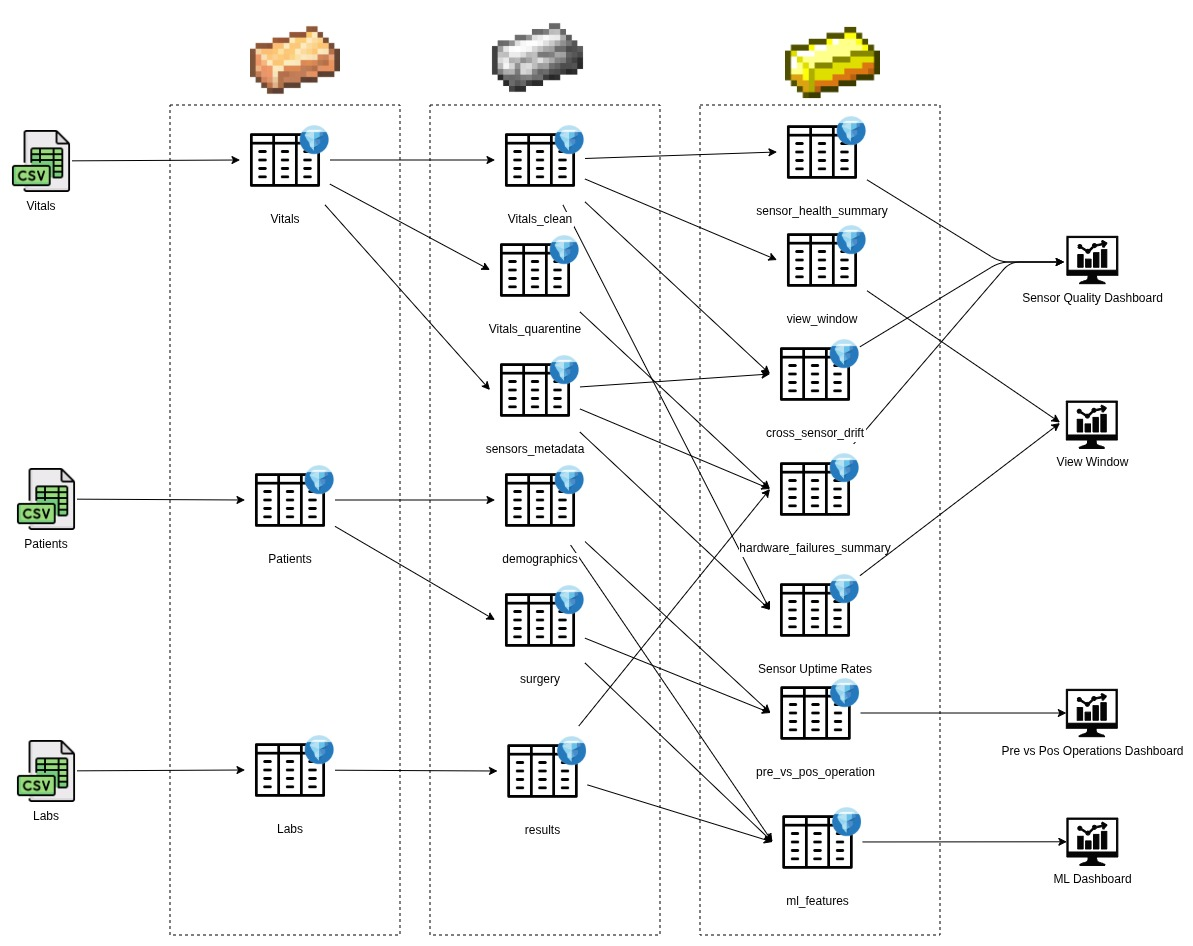
\includegraphics[width=0.75\linewidth]{imagens/architeture.jpg}
	\caption{Representação Gráfica da Arquitetura Medalhão}
	\label{fig:medalioarchiteture}
\end{figure}

\begin{itemize}
	\item \textbf{Camada \textit{Bronze} (Raw):} Atua como a zona de aterragem dos dados. Armazena a informação em estado bruto e imutável, preservando o histórico exato gerado pelos sistemas de origem hospitalar (registos de admissão, resultados laboratoriais e demografia). Os dados csv,  para entrarem nesta camada, primeiro precisam de ser convertidos para o formato \textit{parquet} e \textit{iceberg}.
	
	\item \textbf{Camada \textit{Silver} (Cleansed):} Focada na higienização e conformidade. Nesta camada, os dados brutos são filtrados, padronizados e cruzados. Registos inválidos são tratados e as entidades clínicas são unidas, estabelecendo uma base de dados fiável e relacional (ex: associação do perfil do paciente aos seus exames pré e pós-operatórios).
	
	\item \textbf{Camada \textit{Gold} (Curated):} A camada de consumo analítico. Contém dados altamente refinados e agregados, modelados especificamente para responder às necessidades de negócio. É aqui que reside as tabelas finais, que fornece as métricas pré-calculadas diretamente nos \textit{dashboards}, garantindo máxima performance de leitura.
\end{itemize}


\subsection{Orquestração de Pipelines} \label{subsec:orquestracao_pipelines}

A automatização e gestão dos fluxos de dados (\textit{data pipelines}) são asseguradas pelo \textbf{Flyte}, uma plataforma de orquestração distribuída e tolerante a falhas. O Flyte, embora permita estruturar a lógica de processamento através de Grafos Acíclicos Dirigidos (DAGs), foi impossível executar em modo \textit{"Remote"}, funcionando apenas em modo \textit{"Local"} o que, embora constrangedor, é perfeitamente funcional.

Nesta solução, o \textit{Orquestrator} é responsável por coordenar a transição da informação através do Modelo Medalhão. Ele garante que as tarefas de ingestão (\textit{Bronze}), higienização e cruzamento relacional (\textit{Silver}) e, finalmente, a agregação de métricas clínicas (\textit{Gold}) são executadas com a precedência correta. O uso do Flyte assegura não só a reprodutibilidade dos \textit{workflows}, mas também a robustez do sistema, permitindo a monitorização contínua e a reexecução isolada de tarefas em caso de falhas na infraestrutura.